\chapter{Overview of the UML/MOF Class Diagram Visual Notation}
\label{app:UMLNotation}

This appendix provides a short overview\footnote{A complete discussion on the semantics of UML class diagrams can be found in \cite{Larman}.} of the notation used to represent UML class models and MOF metamodels for readers that are not familiar with object-oriented modelling. Figure \ref{fig:UMLNotation} displays a class diagram that can represent - in different contexts - both a UML model and a MOF metamodel.

\begin{figure}
	\centering
		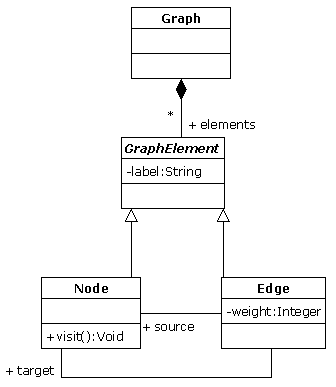
\includegraphics{images/UMLNotation.png}
	\caption{Exemplar Graph UML/MOF Class Diagram}
	\label{fig:UMLNotation}
\end{figure}

\section{Classes, Attributes and Operations}

The model specifies four classes named \emph{Graph}, \emph{GraphElement}, \emph{Node} and \emph{Edge} via boxes. The first compartment of each class-box contains the name of the class. The second and third compartments contain the attributes and the operations of the class respectively. Thus, the \emph{GraphElement} class specifies a \emph{label} attribute of type \emph{String} and the \emph{Edge} class specifies a \emph{weight} attribute of type \emph{Integer}. Also, the \emph{Node} class specifies a parameter-less \emph{visit()} operation. 

\section{Associations and References}

All lines between two boxes that do not end to a white arrowhead represent associations between the respective classes. Each association has two ends (aka references). Each end optionally specifies a name and a multiplicity. Examples of multiplicities are:

\begin{itemize}
	\item \textbf{n} : Exactly n
	\item \textbf{*} : Zero or more
	\item \textbf{+} : One or more
	\item \textbf{n..m} : n to m (inclusive)
	\item \textbf{n..*} : n or more
\end{itemize}

Wherever the multiplicity is not explicit it is assumed to be exactly one\footnote{UML 2.0 Infrastructure, Final adopted specification, pp 121}.

Two different types of associations are used: containment (aka composition) and non-containment. Containment associations are denoted by a black diamond at the side of the container. All other associations are assumed to be non-containment. The semantics of the containment relationship is that a contained instance can only be contained in one container and that if the container is deleted, so are the instances it contains. 

In the example of Figure \ref{fig:UMLNotation}, an instance of \emph{GraphElement} can only be contained in one instance of \emph{Graph}, and if the container \emph{Graph} is deleted from the model, so will the contained instances (\emph{elements}) of \emph{GraphElement}.

There are also two examples of non-containment associations. The \emph{source} and \emph{target} associations between the \emph{Node} and \emph{Edge} class specify that each \emph{Edge} can have exactly one \emph{Node} as \emph{source} and exactly one \emph{Node} as \emph{target} (implicit multiplicities). Since these associations are not containment, deleting an \emph{Edge} does not automatically delete the instances of \emph{Node} that connect to it.

\section{Inheritance and Abstract Classes}

Lines with a white arrowhead between two class-boxes denote an inheritance (subtype) relationship between the respective classes, the class on the side of the arrowhead being the super-type. Both UML and MOF support multiple inheritance and therefore a class can inherit from more than one classes. Classes the name of which appears in \emph{italics} are abstract; i.e. not instantiable. For example, the \emph{GraphElement} in the example is abstract and inherited by the \emph{Node} and \emph{Edge} classes. Combined with the \emph{elements} association from \emph{Graph} to \emph{GraphElement}, it means that the \emph{elements} property of \emph{Graph} can contain both instances of \emph{Edge} and instances of \emph{Node} 

\section{Profiles and Stereotypes}

As UML is a general purpose modelling language it needs to provide a specialization mechanism for expressing domain-related concepts where this is necessary. This mechanism is called a \emph{profile}. In versions 1.x of UML a profile consisted of a set of stereotypes and respective tagged values that could be attached to any model element to specialize it or record additional information. In versions 2.x the profiling mechanism has evolved to allow proper extension of the UML metamodel - a topic which is out of the scope of this discussion. In the examples used in this thesis, the 1.x profiling mechanism is considered. With regard to concrete (graphical) syntax, stereotypes are represented by their name enclosed in $<<$, $>>$. For instance, in Figure \ref{fig:Stereotypes} the \emph{table} stereotype is attached to the Customer UML class to denote that what is modelled is conceptually a database table, instead of a standard object-oriented class, and the \emph{column} stereotype is attached to the \emph{name} attribute to specify that it represents a table column.

\begin{figure}
	\centering
		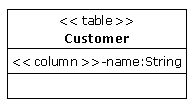
\includegraphics{images/Stereotypes}
	\caption{Exemplar use of UML stereotypes}
	\label{fig:Stereotypes}
\end{figure}




